% ==============================================================================
% SEÇÃO 1: AMBIENTE DE ESTUDO REMOTO E ARQUITETURA HÍBRIDA
% ==============================================================================
\changecolours{ScoutNavy}
\section{Ambiente Remoto e Arquitetura Híbrida}

\begin{frame}{Contexto Pedagógico: Sábado Letivo Autônomo}
  \begin{columns}[T]
    \begin{column}{0.50\textwidth}
      \begin{block}{Objetivo Central da Prática}
        {\footnotesize Dominar CRUD no MongoDB e no Redis, unindo-os através do padrão \textbf{Cache-Aside}.}
      \end{block}
      \vspace{0.2cm}
      {\footnotesize
      \begin{itemize}
        \item \textbf{Nivelamento Prático:} Domínio direto via CLI e GUIs.
        \item \textbf{Arquitetura:} Persistência durável vs RAM de baixa latência.
      \end{itemize}
      }
    \end{column}

    \begin{column}{0.48\textwidth}
      \begin{exampleblock}{Duas Trilhas de Execução}
        {\footnotesize
        \textbf{1. Nuvem + Desktop GUI:}\\
        MongoDB Atlas Free + Compass e Redis Cloud + Redis Insight.\\[6pt]
        \textbf{2. Containers Locais (Docker):}\\
        Provisionamento com comando único:\\[3pt]
        \centering\texttt{docker compose up -d}
        }
      \end{exampleblock}
    \end{column}
  \end{columns}
\end{frame}

\begin{frame}{Opção 1: Setup em Nuvem com GUIs Oficiais}
  \begin{columns}[T]
    \begin{column}{0.50\textwidth}
      \textbf{MongoDB Atlas \& Compass}
      {\footnotesize
      \begin{enumerate}
        \item Criar conta gratuita no \textbf{MongoDB Atlas}.
        \item Criar cluster compartilhado \textbf{M0} (512 MB).
        \item Em \textit{Database Access}, criar usuário/senha.
        \item Em \textit{Network Access}, liberar seu IP (\texttt{0.0.0.0/0}).
        \item Baixar o \textbf{MongoDB Compass} e conectar via string SRV (\texttt{mongodb+srv://...}).
      \end{enumerate}
      }
    \end{column}

    \begin{column}{0.50\textwidth}
      \textbf{Redis Cloud \& Redis Insight}
      {\footnotesize
      \begin{enumerate}
        \item Baixar o \textbf{Redis Insight} (\url{redis.io/insight}).
        \item Conectar em instância local (\texttt{localhost:6379}) ou Redis Cloud gratuito (30 MB).
        \item Acessar navegador de chaves em árvore (\textit{Key Tree}) e terminal CLI integrado.
        \item Analisar estruturas e consumo de memória RAM.
      \end{enumerate}
      }
    \end{column}
  \end{columns}
\end{frame}

\begin{frame}{Opção 2: Setup Local via Docker Compose}
  \begin{columns}[T]
    \begin{column}{0.50\textwidth}
      \begin{exampleblock}{Comando Único de Inicialização}
        {\centering\small\texttt{docker compose up -d}\par}
      \end{exampleblock}
      \vspace{0.2cm}
      {\footnotesize
      \textbf{Serviços Subindo no Host:}
      \begin{itemize}
        \item \textbf{MongoDB 8.0} (\texttt{:27017}) + \textbf{Express} (\texttt{:8081})
        \item \textbf{Redis 7.4} (\texttt{:6379}) + \textbf{Insight} (\texttt{:5540})
      \end{itemize}
      }
    \end{column}

    \begin{column}{0.46\textwidth}
      \begin{block}{Vantagens do Ambiente Local}
        {\footnotesize
        \begin{itemize}
          \item Reprodutível em Linux, Windows e macOS.
          \item Volumes persistentes pré-configurados.
          \item Não polui o sistema operacional host.
          \item Para encerrar: \texttt{docker compose down}.
        \end{itemize}
        }
      \end{block}
    \end{column}
  \end{columns}
\end{frame}

\begin{frame}{Visão Arquitetural Híbrida: MongoDB + Redis}
  \centering
  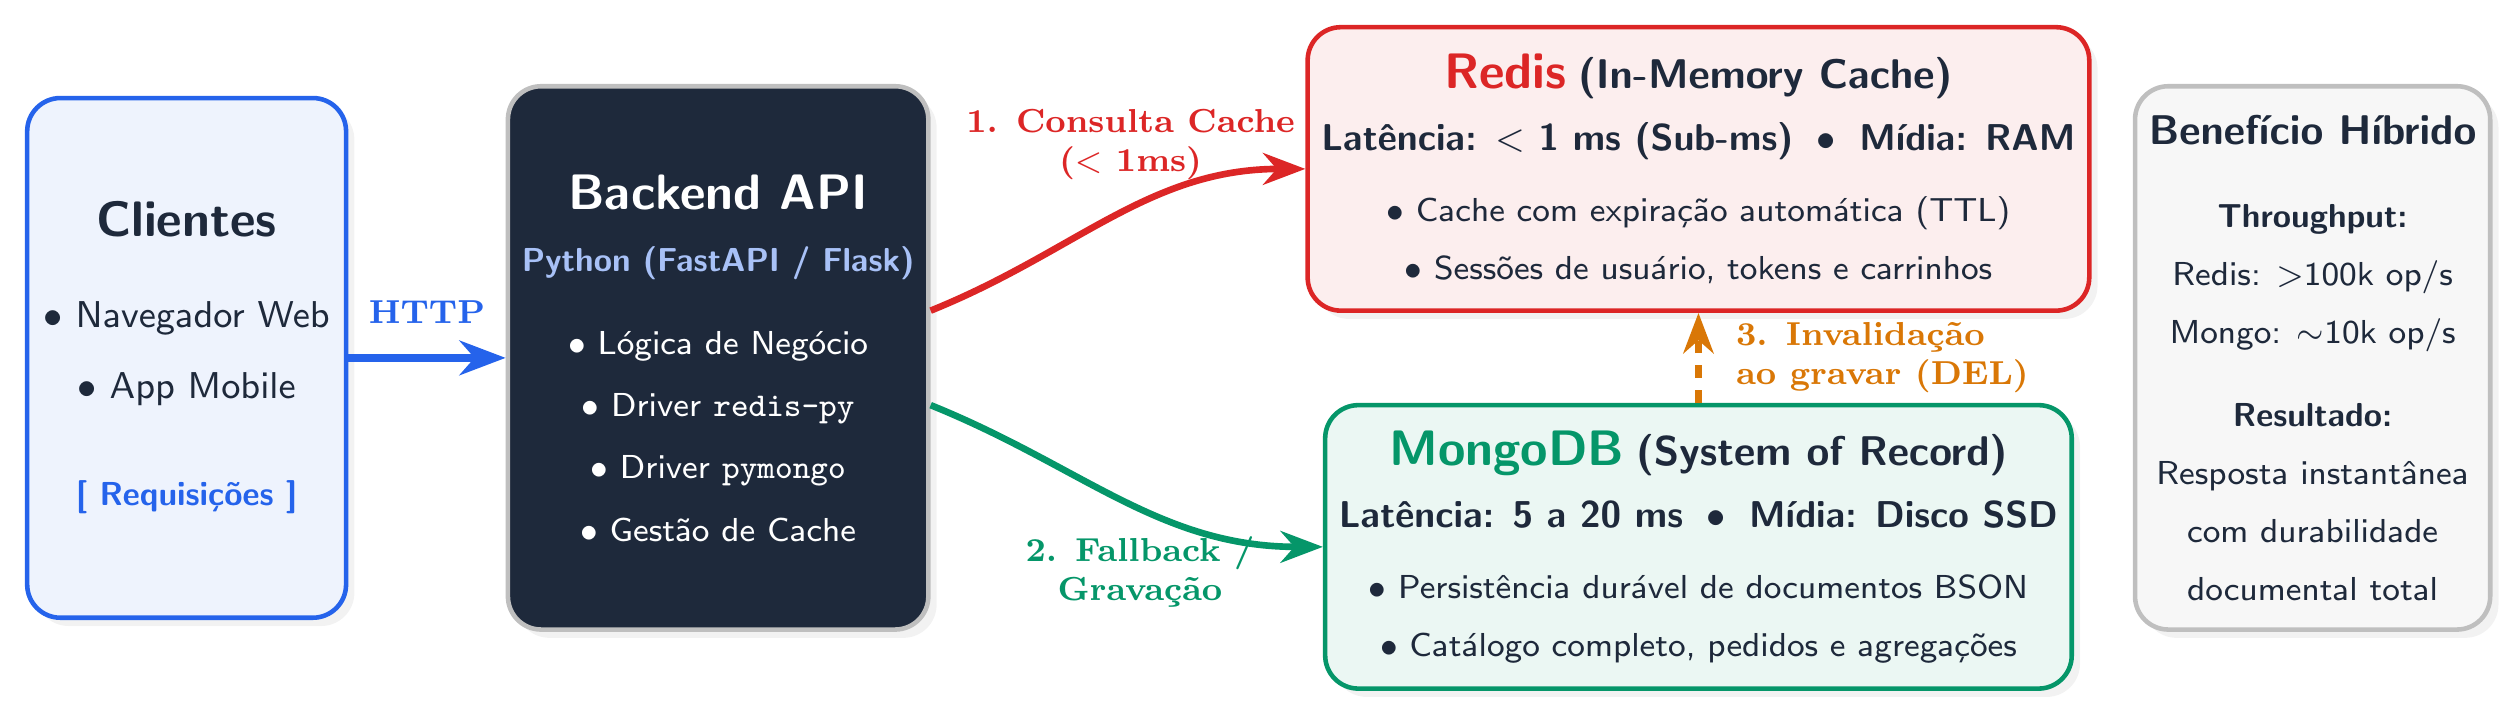
\includegraphics[width=0.98\textwidth,height=0.82\textheight,keepaspectratio]{figuras/fig_arquitetura_hibrida.png}
\end{frame}
